\section{Chroma Subsampling}


\subsection{YCbCr channel decomposition}

\subsubsection{Describe the Cb and Cr channel images. Why do they appear this way?}

Cb is the blue difference chromatic component, and Cr is the red difference chromatic component. Cb contains the difference between blue and the luma component, anc Cr contains the difference between red and the luma component. The Cr image has higher intensities in areas of bright reds in the original image (i.e. the large red bell pepper). The Cb channel has higher intesities in areas where there would be a stronger blue component (i.e. the purple cloth).

\subsubsection{Compare the level of image detail in the Cb and Cr images with the Y channel image. Which contains more fine details? What does that say about the luma (Y) and chroma (Cb and Cr) channels?}

The Y channel contains the most fine image detail. This is because the actual brightness/intensity of an image is contained in the luma channels, while the chroma channels simply provide difference values to allow for proper image coloring. Thus, the luma channel is the most important with regards to image information.

\begin{figure}[ht]
\centering
	\subfigure[Base Image]{
	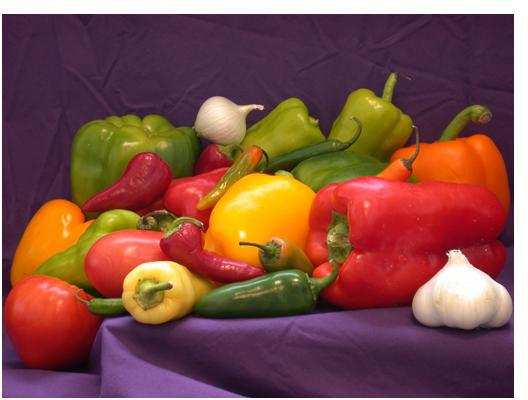
\includegraphics[width=0.45\linewidth]{question2/original_image}
	}
	\subfigure[Luma Component]{
	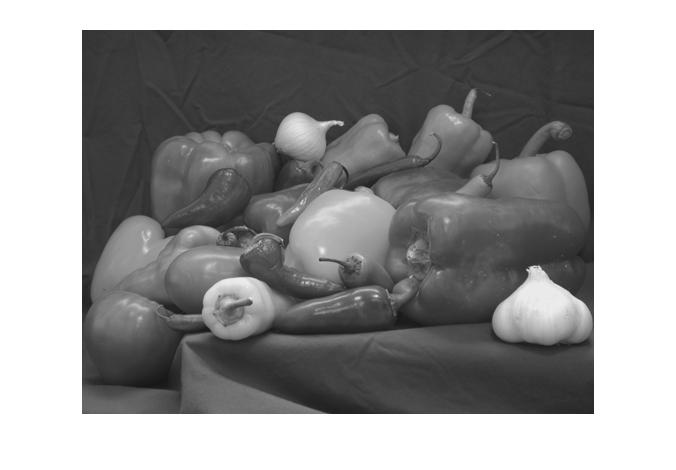
\includegraphics[width=0.45\linewidth]{question2/luma}
	}
	\subfigure[Cb Component]{
	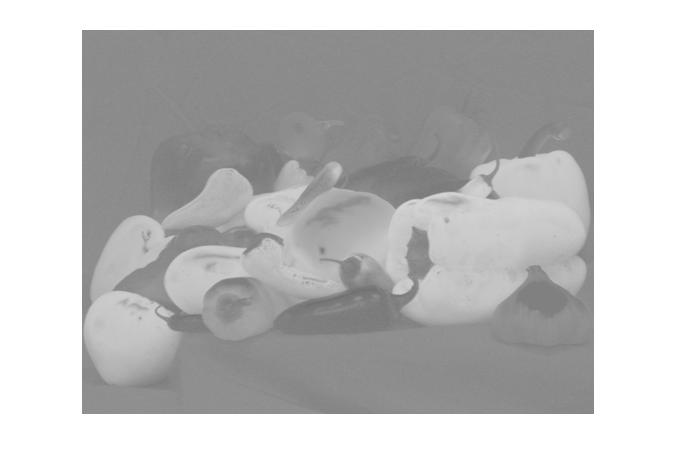
\includegraphics[width=0.45\linewidth]{question2/chroma_cb}
	}
	\subfigure[Cr Component]{
	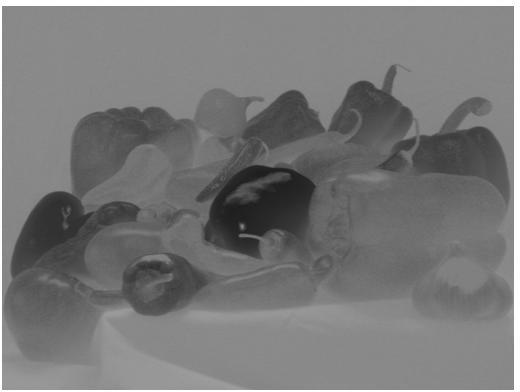
\includegraphics[width=0.45\linewidth]{question2/chroma_cr}
	}
	\caption{YCrCb channels of pepper image}
	\label{fig:noiseGeneration.toy}
\end{figure}
 	
\clearpage
\subsection{Chroma subsampling}
\subsubsection{Compare the resulting image from chroma sub-sampling with the original image. How large are the
visual differences}
The visual differences are essentially non-existant. This is because all of the important information is contained in the luma channel, not the chroma channels.

\begin{figure}[ht]
\centering	
	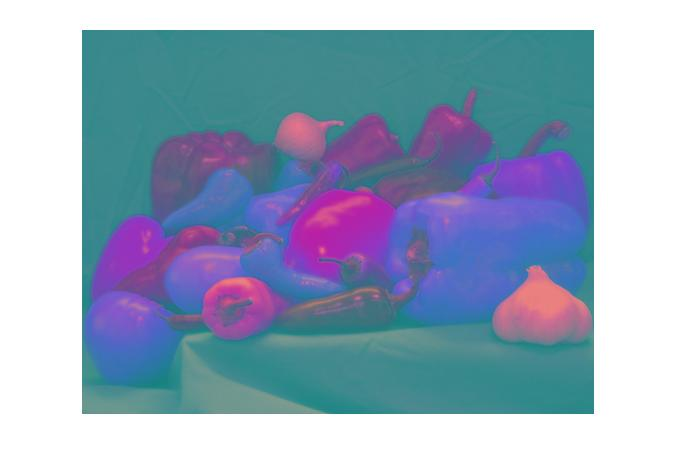
\includegraphics[width=0.65\linewidth]{question2/chroma_subsampled}
	\caption{Chroma subsampled image}
\end{figure}

\subsubsection{Based on the resulting image, what can you say about chroma sub-sampling and its effect on image
quality?}
Based on the subsampled images, it can be said that chroma sub-sampling (at least by a factor of two) has next to no impact on image quality, at least as far as the human eye can detect.

\clearpage
\subsection{Luma subsampling}
\subsubsection{Compare the resulting image from luma sub-sampling with the original image. How large are the
visual differences?}
The visual differences are more pronounced. The luma sub-sampled image is significantly blurrier than the original image.



\begin{figure}[ht]
\centering		
	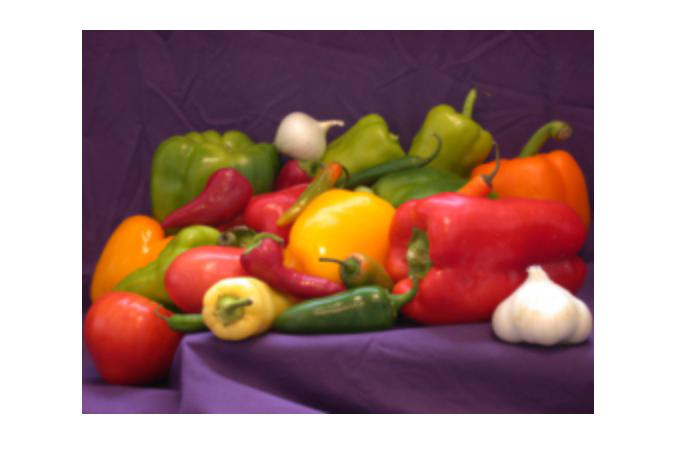
\includegraphics[width=0.65\linewidth]{question2/luma_subsampled}
	\caption{Luma subsampled image}
\end{figure}

\subsubsection{ Compare the resulting image from luma sub-sampling with the image produced using chroma subsampling. Which method performs better? Why}
Chroma subsampling performs significantly better than luma subsampling. This is because not only does undersampling the luma affect the the image through reducing the resolution of the image intensity information, but as the chroma components are the difference between a colour and the luma, information is distorted in those channels as well.


\subsubsection{Based on the resulting image, what can you say about luma sub-sampling and its effect on image
quality}
Luma subsampling has a greater detrimental effect on image quality for reasons stated above.
